\documentclass[11pt]{article}
\usepackage[T1]{fontenc}
\usepackage{lmodern,amsmath,booktabs,graphicx}
\usepackage[margin=1in]{geometry}
\usepackage[colorlinks=true,linkcolor=blue,citecolor=blue,urlcolor=blue]{hyperref}
\hypersetup{pdfauthor={Qianghao Wu},pdftitle={The Zipf law of chess openings on 44.8 million Lichess games: the exponent 2 holds, the finite-size laws do not}}
\title{The Zipf law of chess openings on 44.8 million Lichess games: the exponent 2 holds, the finite-size laws do not}
\author{Qianghao Wu}
\date{November 26, 2026}
\begin{document}
\maketitle
\begin{abstract}
Blasius and T\"onjes (2009) found that the weights of opening lines in a database of 1.4 million chess games follow a Zipf law with the universal exponent $\alpha=2$. Their theory also predicts how the database size $N$ changes the depth-dependent exponents: the slope of $\alpha_d$ against the depth $d$ is $1/\ln N$, and $\alpha_d$ crosses 2 at $d_{\mathrm{cr}}=1+\ln N$. The source tested these finite-size laws at one value of $N$ only. We tested all three predictions out of sample on 44,832,865 rated games from the public Lichess database (2013--2015), with a pre-registered protocol, random subsets from $10^4$ games to the full set, and the authors' own branching model as a known-answer control. The pooled exponent is 2.086 at the full $N$, inside the pre-registered band $2\pm0.10$. The finite-size laws fail. The fitted slope falls with $N$ as $(\ln N)^{-1.76}$, while the same estimator applied to the model gives $(\ln N)^{-0.79}$. The exponent $\alpha_d$ crosses 2 at depth 7.4, while the model gives 17.3. At the source's own sample size the crossing depth is 6.1, against the reported value of about 15. Both failures repeat in every speed, rating and period stratum. A placebo that shuffles moves between games also gives a pooled exponent near 2, so the value 2 alone is not specific to chess. On Lichess, $\alpha_d$ is concave in $d$: its steps are larger than $1/\ln N$ only in the first 7 or 8 plies. These are statements about online play in 2013--2015; we did not re-test the source's database. This work has not yet been reviewed by experts. The computations and the text were produced by AI models (from Anthropic and OpenAI), working under the author's direction.
\end{abstract}
\medskip
\noindent\textit{Keywords:} Zipf's law, chess openings, finite-size scaling, Lichess, pre-registration, replication

\section{Introduction}
A database of chess games defines a tree. Each node is a sequence of the first $d$ half-moves (plies), and its weight $n$ is the number of games that start with that sequence. Blasius and T\"onjes~\cite{bt} counted these weights in ScidBase, a database of $N=1.4\cdot10^6$ games. They found that the number $S(n)$ of nodes with weight $n$, pooled over all depths, follows
\begin{equation}
S(n)\sim n^{-\alpha},\qquad \alpha=2. \label{eq:zipf}
\end{equation}
They explained this law with a multiplicative fragmentation process: a node of weight $n$ passes the fraction $r$ of its games to a child, and $r$ has a fixed distribution $q(r)$. For any well-behaved $q(r)$, the process gives $S(n)\to N/(\mu n^2)$ for $n/N\to0$, with $\mu=\langle-\ln r\rangle$ (their Eq.~8). They measured an arcsine distribution, $q(r)=2/(\pi\sqrt{1-r^2})$, and found it to be depth-independent (their Eq.~2).

The same theory predicts finite-size effects. At depth $d$ the weights follow $S_d(n)\sim n^{-\alpha_d}$ with
\begin{equation}
\alpha_d=(1-\beta)+\frac{d-1}{\ln N}, \label{eq:alphad}
\end{equation}
where $\beta$ is close to 0 (their Eq.~6). So $\alpha_d$ rises linearly in $d$, and the slope $1/\ln N$ falls when the database grows. The depth where $\alpha_d$ crosses 2 is
\begin{equation}
d_{\mathrm{cr}}=1+(1+\beta)\ln N, \label{eq:dcr}
\end{equation}
their Eq.~9. The source writes: ``Applied to the chess database with $N=1.4\cdot10^6$ we obtain $d_{\mathrm{cr}}\approx15$''~\cite{bt}. The value 15 requires the natural logarithm ($1+\ln N=15.15$).

Equations~\eqref{eq:alphad} and~\eqref{eq:dcr} make claims about how the tree changes with $N$. The source tested them at one $N$ only. Maslov's Viewpoint on the paper questioned the pooling of all depths into one distribution and suggested a comparison by player rating~\cite{maslov}. Later work used the same 1.4-million-game database (ChessDB). Perotti, Jo, Schaigorodsky and Billoni modelled the growth of the tree with a nested preferential-growth model~\cite{perotti}. Schaigorodsky, Perotti and Billoni fitted $\alpha_1,\dots,\alpha_4=1.10, 1.29, 1.47, 1.59$ and studied memory effects~\cite{schaig}. Chacoma and Billoni~\cite{chacoma} used 3000 FIDE games and 4000 Lichess games. They drew $n^{-2}$ lines over the popularity distributions and compared the trend of $\alpha_d$ visually with the slope $1/\ln N\approx0.11$ at $N=10^4$. Cheng et al.~\cite{cheng} compared Zipf exponents across rating groups in a Kaggle chess data set and found that they differ. De Marzo and Servedio~\cite{demarzo} studied the network of players and openings on 472,183 Lichess blitz games. None of these works measures $\alpha_d$ or $d_{\mathrm{cr}}$ at several values of $N$. None tests Eq.~\eqref{eq:alphad} or Eq.~\eqref{eq:dcr} out of sample. We found no such test in the citation lists of the source (80 citing works in OpenAlex, 63 in Semantic Scholar) or in searches of arXiv, Zenodo and GitHub (searches of November 24, 2026).

\paragraph{This paper.} The Lichess open database~\cite{lichess} holds every rated game played on the site. Its 36 monthly files for 2013--2015 contain 44.8 million games with moves. That is 32 times the source's $N$. We fixed the tests, the estimator and the decision thresholds in a protocol before we computed any statistic on these games. Table~\ref{tab:tests} gives the outcome. The universal exponent is supported. The two finite-size laws are refuted.

\section{Data and protocol}
\paragraph{Data.} We used the 36 files \texttt{lichess\_db\_standard\_rated\_YYYY-MM.pgn.zst} for 2013-01 to 2015-12 (6.9~GB compressed, CC0). Their SHA-256 sums are in the result folder. The game count published with the files~\cite{lichess} is 45,043,493. Of these, 210,628 games (0.47\%) have no moves. The other 44,832,865 games form the data set.

\paragraph{Pre-registration.} The protocol was committed to the project's git repository on 2026-11-25 at 12:15 CET, before any node weight was computed. The first outcome files were committed at 12:52. The protocol was not changed later. Sections~\ref{sec:robust} and~\ref{sec:explore} report analyses that were not pre-registered, and we mark them as such.

\paragraph{Game key and counting.} A game is reduced to its first 40 plies in standard algebraic notation (SAN), without move numbers, comments, \texttt{!} and \texttt{?}. Transpositions are different nodes, as in the source. We sort the keys and take the longest common prefix of each pair of neighbours; one pass then gives $S_d(n)$ for $d=1,\dots,40$. This is the source's method. A random subset of games keeps the sorted order, so subsets need no new sort.

\paragraph{Estimator.} We used the source's method, least squares on a log-binned histogram. The bin edges are the distinct values of $\lfloor2^{k/2}\rfloor$. A bin enters the fit if its upper edge is at most $N/100$ and it holds at least 5 nodes. The exponent is undefined if fewer than 4 bins enter. The source does not state its fit range; this one was fixed in the protocol.

\paragraph{Statistics.} $\alpha_{\mathrm{pool}}$ is the estimate on the pooled $S(n)$. $b(N)$ is the least-squares slope of $\alpha_d$ on $d$ for $d=3,\dots,\lfloor\ln N\rfloor$. $\rho=b\ln N$; Eq.~\eqref{eq:alphad} predicts $\rho=1$. $\gamma$ is the slope of $\ln b$ on $\ln\ln N$ across the $N$ grid; Eq.~\eqref{eq:alphad} predicts $\gamma=-1$. $d_{\mathrm{cr}}$ is the first depth with $\alpha_d\ge2$, interpolated linearly. The $N$ grid is $10^4, 10^{4.5},\dots,10^{7.5}$, the source's $1.4\cdot10^6$, and the full set. For each $N$ below the full set we drew 5 random subsets (seeds 0--4) and report the mean.

\paragraph{Known-answer control.} The same estimator does not return Eq.~\eqref{eq:alphad} exactly on a finite curve. So the reference for each test is the source's own process passed through the same estimator. We simulated $2\cdot10^6$ chains $n_d=\max(1,\mathrm{round}(n_{d-1}r_d))$ from $n_0=N$, with $r_d$ drawn from the arcsine law, for each $N$ of the grid, and converted the chain counts into expected node counts.

\paragraph{Decision rules.} T1: supported if $|\alpha_{\mathrm{pool}}-2|\le0.10$ at the full $N$. T2: refuted if $|\gamma-\gamma_{\mathrm{model}}|>0.5$ or $|\rho-\rho_{\mathrm{model}}|>0.5\,\rho_{\mathrm{model}}$ at the full $N$; supported if both differences are at most half of these limits. T3: refuted if the slope $s$ of $d_{\mathrm{cr}}$ on $\ln N$ is below 0.5 or above 1.5, or if $d_{\mathrm{cr}}$ differs from the model by more than 4 at the full $N$. The finite-size theory is refuted if T2 or T3 is refuted.

\paragraph{Controls.} Held-out strata at $N=10^6$: Bullet, Blitz and Classical games; terciles of the mean rating (cuts 1534 and 1732); and 2013--2014 against 2015. A placebo: among games with a full 40-ply key, take $1.4\cdot10^6$ games and permute each ply column independently across games (5 seeds). This keeps the move frequencies at each ply and removes all dependence between moves.

\section{Results}
\begin{table}[t]
\centering
\begin{tabular}{llll}
\toprule
Test & Rule & Lichess (model) & Decision\\
\midrule
T1: $\alpha=2$ & $|\alpha_{\mathrm{pool}}-2|\le0.10$ & $\alpha_{\mathrm{pool}}=2.086$ & supported\\
T2: slope $1/\ln N$ & $|\gamma-\gamma_{\mathrm{model}}|\le0.5$ & $\gamma=-1.756\pm0.058$ $(-0.788)$ & refuted\\
 & $|\rho-\rho_{\mathrm{model}}|\le0.5\rho_{\mathrm{model}}$ & $\rho=1.602$ $(1.041)$; rel.\ diff.\ 0.54 & \\
T3: $d_{\mathrm{cr}}=1+\ln N$ & $s\ge0.5$, $|\Delta d_{\mathrm{cr}}|\le4$ & $s=0.400$ $(0.896)$; $d_{\mathrm{cr}}=7.42$ $(17.33)$ & refuted\\
\bottomrule
\end{tabular}
\caption{Pre-registered tests at $N_{\mathrm{full}}=44{,}832{,}865$. Values in brackets come from the authors' model through the same estimator. $\pm$ is the standard deviation of $\gamma$ over the 5 subset seeds. Eq.~\eqref{eq:dcr} with $\beta=0$ gives $d_{\mathrm{cr}}=18.62$ at this $N$.}
\label{tab:tests}
\end{table}

\begin{figure}[t]
\centering
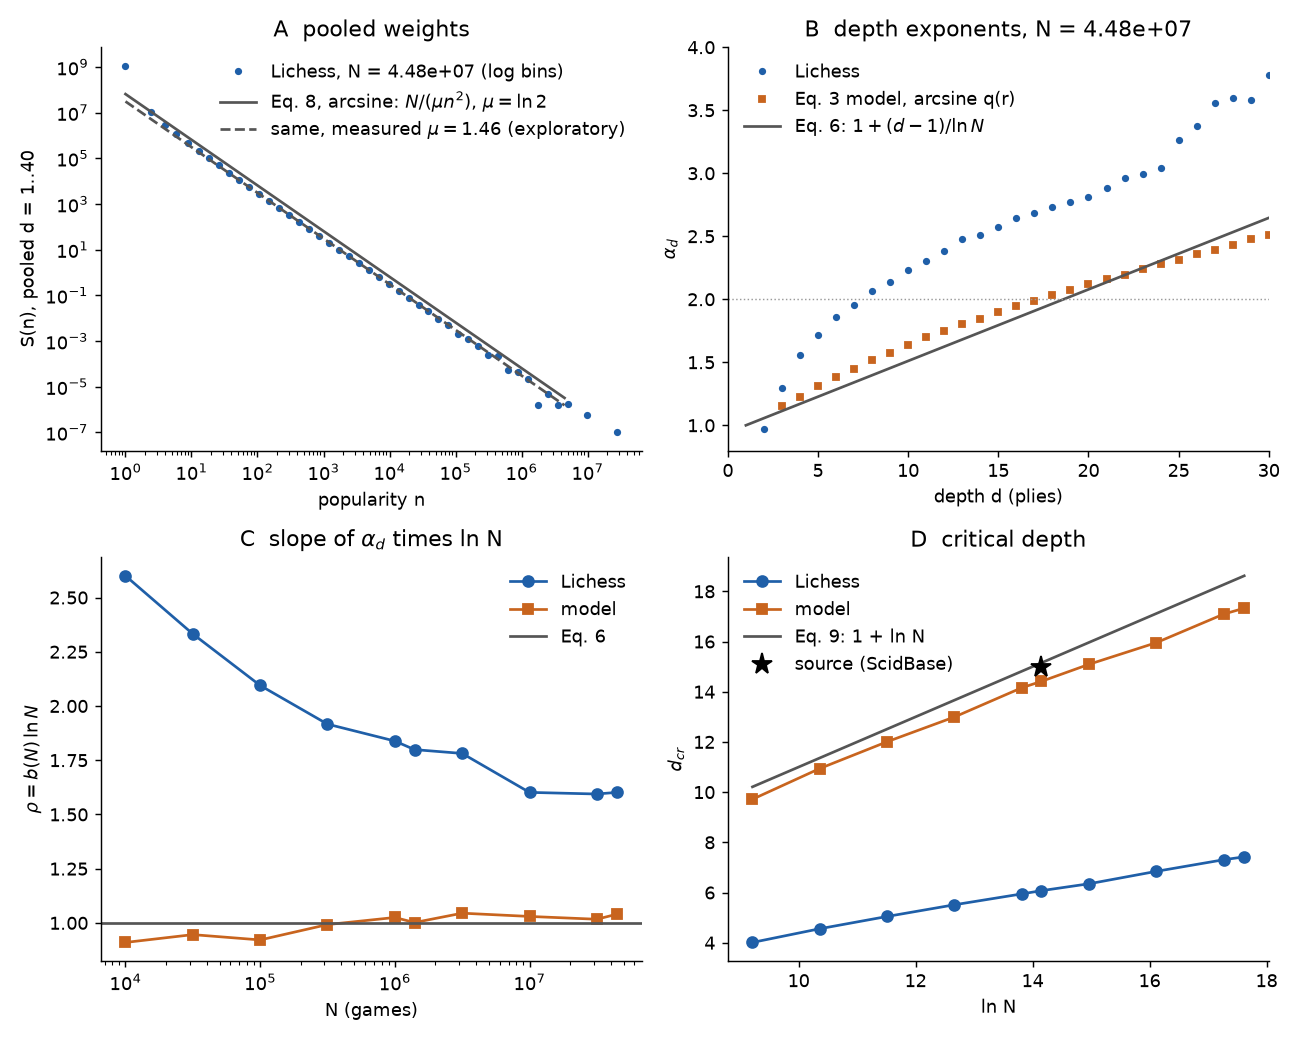
\includegraphics[width=\textwidth]{figures/fig1.png}
\caption{(A) Pooled $S(n)$ at the full $N$, with Eq.~8 of the source for the arcsine value $\mu=\ln2$ (solid) and for the measured $\mu=1.46$ (dashed; exploratory, Section~\ref{sec:explore}). (B) $\alpha_d$ against $d$ for the data, the model and Eq.~\eqref{eq:alphad}. (C) $\rho=b\ln N$ against $N$; Eq.~\eqref{eq:alphad} predicts 1. (D) $d_{\mathrm{cr}}$ against $\ln N$, with the source's value 15 at $N=1.4\cdot10^6$.}
\label{fig:main}
\end{figure}

\begin{table}[t]
\centering
\begin{tabular}{rcccccc}
\toprule
$N$ & $\alpha_{\mathrm{pool}}$ & $b$ & $\rho$ & $d_{\mathrm{cr}}$ & model $\rho$ & model $d_{\mathrm{cr}}$\\
\midrule
$10^4$ & 2.609 & 0.282 & 2.60 & 4.01 & 0.91 & 9.72\\
$10^5$ & 2.299 & 0.182 & 2.09 & 5.05 & 0.92 & 12.01\\
$10^6$ & 2.166 & 0.133 & 1.84 & 5.95 & 1.03 & 14.16\\
$1.4\cdot10^6$ & 2.155 & 0.127 & 1.80 & 6.07 & 1.00 & 14.41\\
$10^7$ & 2.105 & 0.099 & 1.60 & 6.85 & 1.03 & 15.96\\
$4.48\cdot10^7$ & 2.086 & 0.091 & 1.60 & 7.42 & 1.04 & 17.33\\
\bottomrule
\end{tabular}
\caption{Statistics at selected $N$ (mean of 5 random subsets below the full set). $1+\ln N$ is 10.21, 12.51, 14.82, 15.15, 17.12 and 18.62 on these rows.}
\label{tab:grid}
\end{table}

\paragraph{T1: the pooled exponent.} At the full $N$, $\alpha_{\mathrm{pool}}=2.086$. T1 is supported. The pooled exponent falls toward 2 as $N$ grows: 2.61 at $10^4$ and 2.09 at $4.5\cdot10^7$ (Table~\ref{tab:grid}). The model shows the same finite-size trend, from 2.41 to 2.04. A Clauset--Shalizi--Newman fit~\cite{csn} with the \texttt{powerlaw} package~\cite{powerlaw}, at $N=1.4\cdot10^6$ (seed 0), gives $x_{\min}=16$ (KS distance 0.0025), $\alpha=2.024$ and 62,030 nodes in the tail. The likelihood ratio does not prefer a lognormal ($R=0.98$, $p=0.33$) or a truncated power law ($R=-0.72$, $p=0.47$). The pooled weights are nested, so these $p$-values are descriptive only.

\paragraph{T2: the slope of $\alpha_d$.} The estimator recovers Eq.~\eqref{eq:alphad} on the model: $\rho_{\mathrm{model}}$ is between 0.91 and 1.04 on the whole grid. On Lichess, $\rho$ is 2.60 at $10^4$ and 1.60 at the full $N$. The slope falls faster than $1/\ln N$: $\gamma=-1.756$ (SD 0.058 over 5 seeds) against $-0.788$ for the model. Both T2 limits are exceeded. T2 is refuted.

\paragraph{T3: the crossing depth.} On the model, $d_{\mathrm{cr}}$ grows with slope 0.90 in $\ln N$, close to Eq.~\eqref{eq:dcr}. On Lichess the slope is 0.40, and $d_{\mathrm{cr}}=7.42$ at the full $N$, against 17.33 for the model and 18.62 for Eq.~\eqref{eq:dcr}. At the source's $N=1.4\cdot10^6$, Lichess gives $d_{\mathrm{cr}}=6.1$; the source reports about 15 for ScidBase. T3 is refuted.

\paragraph{Held-out strata.} Table~\ref{tab:strata} gives the strata at $N=10^6$. No stratum meets the pre-registered replication rule. In all strata, $\alpha_{\mathrm{pool}}$ is 2.155--2.167. The full set gives 2.166 at the same $N$, so this is the finite-size trend of T1 and not a difference between strata. The T2 and T3 failures repeat in every stratum: $\rho\ge1.68$ against $\rho_{\mathrm{model}}(10^6)=1.03$, and $d_{\mathrm{cr}}\le6.4$ against 14.2. The deviation is smallest for high ratings and Blitz and largest for Bullet and low ratings.

\begin{table}[t]
\centering
\begin{tabular}{lrccc}
\toprule
Stratum & games & $\alpha_{\mathrm{pool}}$ & $\rho$ & $d_{\mathrm{cr}}$\\
\midrule
Bullet & 14,337,880 & 2.155 & 2.16 & 5.69\\
Blitz & 18,281,202 & 2.164 & 1.70 & 6.27\\
Classical & 11,582,480 & 2.161 & 1.86 & 6.10\\
Rating $<1534$ & 14,901,926 & 2.164 & 2.08 & 5.75\\
Rating 1534--1731 & 14,983,580 & 2.162 & 1.89 & 6.02\\
Rating $\ge1732$ & 14,942,928 & 2.158 & 1.68 & 6.38\\
2013--2014 & 14,964,152 & 2.167 & 1.89 & 5.89\\
2015 & 29,868,713 & 2.164 & 1.84 & 5.97\\
\bottomrule
\end{tabular}
\caption{Held-out strata, $N=10^6$ games each, mean of 5 subsets.}
\label{tab:strata}
\end{table}

\paragraph{Placebo.} The placebo uses the 36,705,863 games with a full 40-ply key. On the real games ($1.4\cdot10^6$, mean of 5 seeds) we get $\alpha_{\mathrm{pool}}=2.155$, $b=0.128$, $\rho=1.81$ and $d_{\mathrm{cr}}=6.07$. On the shuffled games, $\alpha_{\mathrm{pool}}$ is 2.137--2.138, $b$ is 0.75--0.79 and $\rho$ is 10.6--11.1 over the 5 seeds. So the shuffled tree also gives a pooled exponent near 2. This agrees with the source's argument that any well-behaved branching process gives $\alpha=2$. It also means that $\alpha\approx2$ alone does not show anything specific to chess. The shuffle makes $b$ about 6 times larger. In the shuffled set $\alpha_d$ is defined at only 6 depths, so we use only this ratio and not the exact shuffled value.

\section{Robustness of T2 and T3 (not pre-registered)}\label{sec:robust}
The fit range of the estimator is our choice, because the source does not state one. An independent robustness script repeats T2 and T3 with five fit ranges, new random subsets (seeds 9000--9002, 3 per $N$) and a separately written estimator. Table~\ref{tab:robust} gives the result. The first row uses the protocol range. Its $\gamma=-1.82$ differs from the pre-registered $-1.756$ only because the subsets are new; $\rho$ and $d_{\mathrm{cr}}$ at the full $N$ use all games and are equal in both analyses.

\begin{table}[t]
\centering\small
\begin{tabular}{llccccc}
\toprule
lowest $n$ & highest $n$ & $\gamma$ & $\rho$ & $d_{\mathrm{cr}}$ & T2 & T3\\
\midrule
1 (protocol) & $N/100$ (protocol) & $-1.82$ $(-0.78)$ & 1.60 (1.05) & 7.42 (17.33) & refuted & refuted\\
2 & $N/100$ & $-1.56$ $(-0.79)$ & 1.47 (1.06) & 7.38 (17.40) & refuted & refuted\\
4 & $N/100$ & $-1.31$ $(-0.81)$ & 1.43 (1.07) & 7.31 (17.18) & inconclusive & refuted\\
1 & $N/1000$ & $-1.89$ $(-0.98)$ & 1.73 (1.00) & 7.83 (18.10) & refuted & refuted\\
2 & $N/10$ & $-1.59$ $(-0.86)$ & 1.45 (1.05) & 7.38 (17.40) & refuted & refuted\\
\bottomrule
\end{tabular}
\caption{T2 and T3 for five fit ranges at the full $N$; model values in brackets. Decisions use the pre-registered thresholds.}
\label{tab:robust}
\end{table}

T3 is refuted in all five fit ranges. The slope of $d_{\mathrm{cr}}$ on $\ln N$ is 0.37--0.43 (model 0.78--1.12). T2 changes to ``inconclusive'' for one range (lowest weight 4: $|\gamma-\gamma_{\mathrm{model}}|=0.499$, relative $\rho$ difference 0.33).

The reason is the shape of $\alpha_d$. On Lichess it is concave in $d$, not linear. At the full $N$ (protocol range), $\alpha_2,\dots,\alpha_9$ are 0.97, 1.30, 1.55, 1.72, 1.86, 1.95, 2.06 and 2.14. After that, the steps are about 0.05 to 0.09. Eq.~\eqref{eq:alphad} predicts a straight line with slope $1/\ln N=0.057$. Thus the value of $b$ depends on the depth window, and the protocol window $3\le d\le\lfloor\ln N\rfloor$ grows with $N$, which adds to $\gamma$. In the fixed window $d=3,\dots,9$, $\gamma=-1.13$ (model $-0.46$) and $\rho=2.38$ (model 1.29); T2 is still refuted by the same thresholds. In the window $d\ge8$ (lowest weight 2), $\rho=1.03$ (model 0.92). So the slope at depths 8 and more is close to $1/\ln N$, and the excess slope is in the first 7 or 8 plies.

The published exponents for ChessDB show the same feature. The values $\alpha_1,\dots,\alpha_4$ (1.10, 1.29, 1.47 and 1.59) of Schaigorodsky et al.~\cite{schaig} have steps 0.19, 0.18 and 0.12, while $1/\ln N=0.071$ at $N=1.4\cdot10^6$. This is our reading of their numbers. Their fit method differs from ours, so it is not a test.

T3 fixes $\beta=0$, as the source does for $d_{\mathrm{cr}}\approx15$. With a free $\beta$, the measured slope $s=0.40$ equals Eq.~\eqref{eq:dcr} with $\beta\approx-0.6$. But Eq.~\eqref{eq:alphad} with the same $\beta$ predicts a straight line that starts at $\alpha_2\approx1.66$. The data give $\alpha_2=0.97$ and a concave curve. So no single $\beta$ makes Eq.~\eqref{eq:alphad} and Eq.~\eqref{eq:dcr} agree with the data together. This is a reading of the numbers above, not a pre-registered test.

\section{Exploratory: branching ratios (not pre-registered)}\label{sec:explore}
We measured the branching ratios $r$ as in Fig.~3A of the source (parents with $n\ge100$, each edge weighted by $r$). The mean $\mu=\langle-\ln r\rangle$ is 1.47 at $N=1.4\cdot10^6$ and 1.46 at $N=10^{6.5}$. The arcsine law gives $\mu=\ln2=0.69$. At $N=1.4\cdot10^6$ the value is highest at ply 2 (2.06) and falls with depth (1.16--1.26 at plies 12--14). So Lichess games split faster than the arcsine law, and the split rate depends on depth. With the measured $\mu=1.46$, Eq.~8 of the source matches the amplitude of the pooled $S(n)$ (Fig.~\ref{fig:main}A).

To separate the depth dependence from correlations along a game, we shuffled the measured ratios across games within each depth and rebuilt the chains. This surrogate gives $d_{\mathrm{cr}}=6.4$ ($N=1.4\cdot10^6$) and 6.8 ($N=10^{6.5}$), close to the data (6.1 and 6.4). It gives $\rho=1.15$ and 1.25, between the model (1.0) and the data (1.8). One reading: the early crossing follows from the fast, depth-dependent splitting, and the excess slope comes partly from correlations along the path of a game. No pre-registered test supports this reading.

\section{How the result was checked}
\begin{itemize}
\item \textbf{Full rerun.} \texttt{checks/rerun.py} checks the SHA-256 of the 36 raw files (it downloads missing files), parses them, builds the sorted key set, runs all pre-registered stages, the robustness script and the exploratory analysis, draws Fig.~\ref{fig:main}, and compares 1950 numbers with \texttt{data/expected.json} (relative tolerance $10^{-6}$). The script refuses a work folder that already holds parsed or built data, so each run starts from the raw files. Three from-zero runs before release (one by the solving agent, one by the verifying agent, one on the released folder) printed \texttt{1950/1950 numbers match}.
\item \textbf{Counting code.} \texttt{checks/test\_counting.py} counts $10^5$ synthetic games with the sort/LCP code and with a direct prefix dictionary. The histograms are equal at all 40 depths, for the full set and for a subset.
\item \textbf{Independent count.} A second program, written separately by the verifying agent, parses the raw PGN text with its own SAN regular expression, hashes each prefix and counts with \texttt{numpy.unique}. On all 36 months it finds the same 44,832,865 games, $S_d(n)$ equal to ours at depths 1 to 12, and $d_{\mathrm{cr}}=7.4214$ with its own estimator. Depths 13 to 40 were checked independently on one month only.
\item \textbf{Protocol order.} The protocol commit precedes all outcome files, and the protocol file has no later change.
\end{itemize}

\section{Limits}
\begin{itemize}
\item \textbf{Population.} Lichess in 2013--2015 is online play, mostly Bullet and Blitz, with mean ratings near 1500--1800. ScidBase holds mostly master and club games. The refutation concerns Eqs.~\eqref{eq:alphad} and~\eqref{eq:dcr} as general laws of opening trees. It does not show that the source's measurements on ScidBase are wrong. We had no ScidBase data and did not re-test them. Even the top rating tercile and Classical games give $d_{\mathrm{cr}}\approx6.1$--6.4 at $N=10^6$, and no stratum here is comparable to master play.
\item \textbf{Estimator.} The fit range is ours. T3 does not depend on it in five ranges. T2 is refuted in four of five ranges and inconclusive in one.
\item \textbf{$\beta$.} T3 tests Eq.~\eqref{eq:dcr} with $\beta=0$ only.
\item \textbf{Statistics.} The CSN $p$-values treat nested weights as independent. Sections~\ref{sec:robust} and~\ref{sec:explore} are not pre-registered.
\item \textbf{Earlier work.} Chacoma and Billoni~\cite{chacoma} report that the trend of $\alpha_d$ on their mixed set of $10^4$ games agrees with slope 0.11. On Lichess subsets of $10^4$ games we get $b=0.28$. Their data (FIDE games and Lichess games above 2500 and below 1500, all classical) and their fits differ from ours. We did not find the cause of the difference.
\item \textbf{Keys.} We did not check the SAN text for legality. We assume that the Lichess server records only legal moves. Games with no moves (0.47\%) are dropped.
\end{itemize}

\section{Conclusion}
On 44.8 million Lichess games the pooled weights of opening lines have exponent 2.09, which supports the universal $\alpha=2$. A shuffled placebo also gives an exponent near 2, as the theory of the source predicts for any branching process. The finite-size laws of the same theory fail on this data: the slope of $\alpha_d$ falls faster than $1/\ln N$, $\alpha_d$ is concave in $d$, and $\alpha_d$ crosses 2 at about depth 7, not near $1+\ln N\approx18$. Both failures hold in every stratum and, for $d_{\mathrm{cr}}$, in every fit range.

\begin{thebibliography}{10}
\bibitem{bt} B. Blasius and R. T\"onjes, ``Zipf's law in the popularity distribution of chess openings,'' \emph{Phys. Rev. Lett.} \textbf{103}, 218701 (2009). \href{https://doi.org/10.1103/PhysRevLett.103.218701}{doi:10.1103/PhysRevLett.103.218701}; \href{https://arxiv.org/abs/0704.2711}{arXiv:0704.2711v2}.
\bibitem{maslov} S. Maslov, ``Power laws in chess,'' \emph{Physics} \textbf{2}, 97 (2009). \href{https://doi.org/10.1103/Physics.2.97}{doi:10.1103/Physics.2.97}.
\bibitem{perotti} J. I. Perotti, H.-H. Jo, A. L. Schaigorodsky and O. V. Billoni, ``Innovation and nested preferential growth in chess playing behavior,'' \emph{EPL} \textbf{104}, 48005 (2013). \href{https://doi.org/10.1209/0295-5075/104/48005}{doi:10.1209/0295-5075/104/48005}.
\bibitem{schaig} A. L. Schaigorodsky, J. I. Perotti and O. V. Billoni, ``A study of memory effects in a chess database,'' \emph{PLoS ONE} \textbf{11}, e0168213 (2016), Fig.~1 caption. \href{https://doi.org/10.1371/journal.pone.0168213}{doi:10.1371/journal.pone.0168213}.
\bibitem{chacoma} A. Chacoma and O. V. Billoni, ``Emergent complexity in the decision-making process of chess players,'' \emph{Sci. Rep.} \textbf{15}, 23234 (2025). \href{https://doi.org/10.1038/s41598-025-06335-9}{doi:10.1038/s41598-025-06335-9}.
\bibitem{cheng} Y. Cheng, Z. Fang, D. Xu, Y. Dong, X. Hu and J. Qian, ``Multi-scaling laws and long-term correlations in chess game records popularity,'' \emph{J. East China Normal Univ. (Nat. Sci.)} 2025(3), 137--146. \href{https://doi.org/10.3969/j.issn.1000-5641.2025.03.016}{doi:10.3969/j.issn.1000-5641.2025.03.016}.
\bibitem{demarzo} G. De Marzo and V. D. P. Servedio, ``Quantifying the complexity and similarity of chess openings using online chess community data,'' \emph{Sci. Rep.} \textbf{13}, 5327 (2023). \href{https://doi.org/10.1038/s41598-023-31658-w}{doi:10.1038/s41598-023-31658-w}.
\bibitem{csn} A. Clauset, C. R. Shalizi and M. E. J. Newman, ``Power-law distributions in empirical data,'' \emph{SIAM Rev.} \textbf{51}, 661--703 (2009). \href{https://doi.org/10.1137/070710111}{doi:10.1137/070710111}.
\bibitem{powerlaw} J. Alstott, E. Bullmore and D. Plenz, ``powerlaw: a Python package for analysis of heavy-tailed distributions,'' \emph{PLoS ONE} \textbf{9}, e85777 (2014). \href{https://doi.org/10.1371/journal.pone.0085777}{doi:10.1371/journal.pone.0085777}.
\bibitem{lichess} Lichess, \emph{lichess.org open database}, standard rated games 2013-01 to 2015-12, \url{https://database.lichess.org/}, CC0, accessed November 25, 2026.
\end{thebibliography}
\end{document}
